\documentclass[12pt]{article}
\usepackage[margin=1in]{geometry}
\usepackage{amsmath}
\usepackage{amssymb}
\usepackage{graphicx}
\usepackage{booktabs}
\usepackage{float}
\usepackage{caption}

\setlength{\parindent}{0pt}
\setlength{\parskip}{8pt}

\title{CS 440: Introduction to Artificial Intelligence\\Assignment 1 --- Fast Trajectory Replanning}
\author{Sadhana Vasanthakumar (RUID: 233000133)\\
Sonakshi Sharma (RUID: 229005962)\\
Simone S Chanekar (RUID: 217006428)}
\date{February 2026}

\begin{document}

\maketitle

% -------------------------------------------------------
\section*{Part 0: Environment Setup}

We generated 50 gridworlds of size $101 \times 101$ using a depth-first search algorithm with random tie-breaking. The generation works as follows. All cells start as unvisited. A random starting cell is selected, marked as visited and unblocked (value 0). From that cell, we randomly pick an unvisited neighbor. With 30\% probability the neighbor is marked blocked (value 1) and with 70\% probability it is marked unblocked and pushed onto a stack.

When the current cell has no unvisited neighbors, we backtrack by popping the stack. If the stack empties before all cells are visited, we restart from a random unvisited cell. This continues until every cell is visited. Finally, the start cell $(0,0)$ and goal cell $(100,100)$ are forced to be unblocked.

The 50 mazes are stored together in a single JSON file (\texttt{mazes.json}) as a list of $101 \times 101$ grids of integers (0 = free, 1 = blocked). The implementation is in \texttt{create\_grid\_worlds.py}, and the three search algorithms are in \texttt{q2.py}, \texttt{q3.py}, and \texttt{q5.py}. A custom binary min-heap is implemented from scratch in \texttt{custom\_pq.py} with two classes: \texttt{CustomPQ\_maxG} (breaks ties by largest $g$-value) and \texttt{CustomPQ\_minG} (breaks ties by smallest $g$-value).

Of the 50 generated mazes, 19 are solvable and 31 are not. The high unsolvable rate reflects the 30\% blocking probability, which frequently creates disconnected regions separating the start from the goal.

\begin{figure}[H]
  \centering
  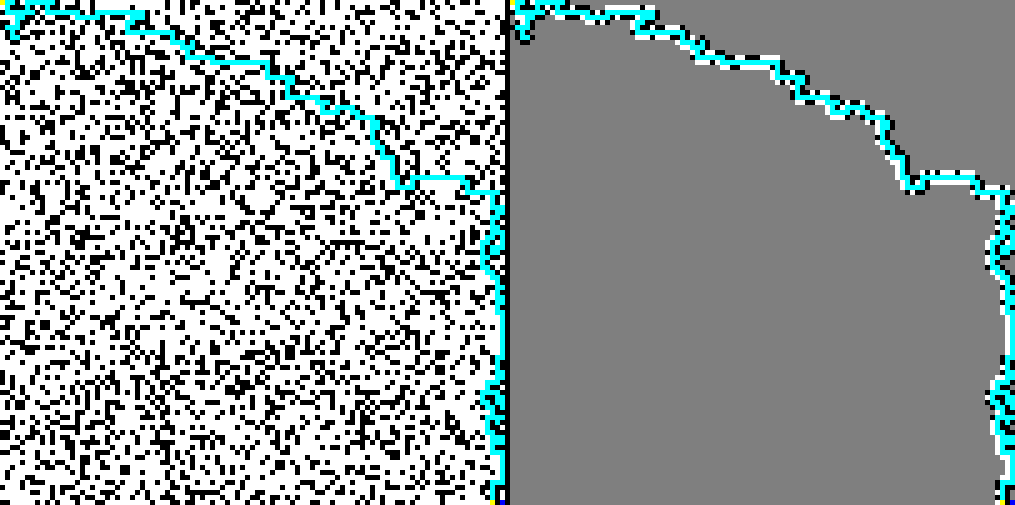
\includegraphics[width=0.85\textwidth]{q2-vis.png}
  \caption{Visualization of Repeated Forward A* (max\_g) on maze 3. Left: the full ground-truth maze with the executed path shown in cyan. Right: the agent's knowledge during the run --- grey cells are unseen (assumed free), white cells are known free, black cells are known blocked, and the cyan path shows where the agent actually moved.}
\end{figure}

% -------------------------------------------------------
\section*{Part 1: Understanding the Methods}

\subsection*{(a) Why the Agent Moves East First}

In Figure 8, the agent is at cell E2 and the target is at E5. The agent does not know which cells are blocked, so it assumes all unseen cells are free (the freespace assumption). Using Manhattan distance as the heuristic $h$:

\begin{itemize}
  \item \textbf{Move east to E3:} $g = 1$, $h = |E - E| + |3 - 5| = 2$, so $f = 3$.
  \item \textbf{Move north to D2:} $g = 1$, $h = |D - E| + |2 - 5| = 1 + 3 = 4$, so $f = 5$.
\end{itemize}

A* always expands the cell with the lowest $f$-value first. Since moving east gives $f = 3$ and moving north gives $f = 5$, the agent moves east. Intuitively, moving east keeps the agent on the same row as the target, whereas moving north takes it further away.

\subsection*{(b) Finite Time Guarantee and Upper Bound}

\textbf{Claim:} In a finite gridworld, the agent either reaches the target or determines it is impossible in finite time, and the number of moves is bounded by $n^2$ where $n$ is the number of unblocked cells.

\textbf{Argument:} The gridworld has finitely many cells, so there are finitely many possible blocked/unblocked configurations the agent can discover. Each time the agent moves to a new cell, it observes its four neighbors and adds any blocked ones to its known-blocked set. This set only grows --- blocked cells are never removed. Since there are at most $n$ unblocked cells, after at most $n$ discoveries the agent's knowledge stabilizes.

Each A* search either finds a path or proves that no path exists given the currently known blocked cells. If a path is found, the agent follows it until it reaches the goal or hits a newly discovered blocked cell. Every time a block is discovered, at least one new cell is added to the known-blocked set. Since there are only finitely many cells, this can happen at most a finite number of times.

\textbf{Upper bound:} Let $n$ be the number of unblocked cells. In the worst case, the agent moves up to $n$ steps before discovering a new blocked cell, and this replanning can happen at most $n$ times (once per unblocked cell on the path). Therefore the total number of moves is at most $n \times n = n^2$.

% -------------------------------------------------------
\section*{Part 2: Effects of Tie Breaking}

When multiple cells in the open list share the same $f$-value, the algorithm must decide which to expand first. We compared two strategies: breaking ties in favor of larger $g$-values (max\_g) versus smaller $g$-values (min\_g). Both were tested on all 50 mazes.

\textbf{Results:}

\begin{table}[H]
\centering
\begin{tabular}{lrrr}
\toprule
\textbf{Strategy} & \textbf{Avg.\ Expansions} & \textbf{Avg.\ Runtime (ms)} & \textbf{Mazes Won} \\
\midrule
max\_g (larger $g$) & 7,346 & 45.6 & 42/50 \\
min\_g (smaller $g$) & 161,116 & 762.1 & 8/50 \\
\bottomrule
\end{tabular}
\caption{Tie-breaking comparison over 50 mazes. Both strategies solved the same 19 mazes. The 8 ``wins'' for min\_g are ties on unsolvable mazes where both strategies expand identically.}
\end{table}

\textbf{Observation:} max\_g expands roughly \textbf{21.9 times fewer cells} than min\_g and is about 16 times faster on average.

\textbf{Explanation:} When two cells have the same $f = g + h$ value, a larger $g$ means a smaller $h$ --- meaning that cell is estimated to be closer to the goal. Breaking ties in favor of larger $g$ therefore pushes the search toward the goal, keeping it focused. Breaking ties in favor of smaller $g$ favors cells closer to the start, causing the search to spread broadly across the grid before making real progress toward the goal. This broad spreading wastes enormous effort expanding cells that are far from the optimal path.

% -------------------------------------------------------
\section*{Part 3: Forward vs.\ Backward A*}

Repeated Forward A* searches from the agent's current position to the goal. Repeated Backward A* searches from the goal back to the agent's current position, using the agent's position as the ``goal'' of the A* search. Both used max\_g tie-breaking.

\textbf{Results:}

\begin{table}[H]
\centering
\begin{tabular}{lrrr}
\toprule
\textbf{Algorithm} & \textbf{Avg.\ Expansions} & \textbf{Avg.\ Runtime (ms)} & \textbf{Mazes Won} \\
\midrule
Repeated Forward A* & 7,346 & 44.0 & 50/50 \\
Repeated Backward A* & 85,185 & 897.4 & 0/50 \\
\bottomrule
\end{tabular}
\caption{Forward vs.\ Backward A* over 50 mazes. Both solved the same 19 mazes.}
\end{table}

\textbf{Observation:} Forward A* outperforms Backward A* in \textbf{every single maze}, expanding 11.6 times fewer cells on average.

\textbf{Explanation:} The key difference is in the heuristic. In Forward A*, the heuristic $h(s) = \text{manhattan}(s,\, \text{goal})$ estimates distance to the fixed target. Since the target never moves, this heuristic remains meaningful across all replanning episodes. In Backward A*, the heuristic estimates distance to the agent's current position, which changes every time the agent moves. This means the heuristic target keeps shifting, making the estimates less reliable from one replan to the next. The result is that Backward A* explores many more cells per search before finding a path, because its heuristic cannot guide it as effectively.

% -------------------------------------------------------
\section*{Part 4: Heuristics in Adaptive A*}

\subsection*{(a) Manhattan Distance is Consistent}

A heuristic $h$ is \textit{consistent} (also called monotone) if:
\[h(\text{goal}) = 0 \quad \text{and} \quad h(s) \leq c(s, a) + h(s') \quad \text{for all states } s, s'\]
where $s'$ is the successor of $s$ under action $a$ with cost $c(s,a)$.

For Manhattan distance in a 4-directional gridworld, $h(s) = |r_s - r_g| + |c_s - c_g|$ where $(r_g, c_g)$ is the goal cell. Clearly $h(\text{goal}) = 0$.

Each move changes exactly one coordinate by exactly 1. If the move brings the agent closer to the goal along that coordinate, $h$ decreases by 1, so $h(s) = 1 + h(s')$. If the move takes the agent away, $h$ increases by 1, so $h(s) = h(s') - 1 < 1 + h(s')$. In both cases $h(s) \leq 1 + h(s') = c(s,a) + h(s')$, which is exactly the consistency condition.

\subsection*{(b) Adaptive A* Preserves Consistency}

After an A* search finds a path with goal cost $g(\text{goal})$, Adaptive A* updates the h-value of every expanded state $s$ as:
\[h_\text{new}(s) = g(\text{goal}) - g(s)\]

\textbf{Admissibility:} Since $g(\text{goal})$ is the true shortest-path cost from start to goal, and $g(s)$ is the shortest-path cost from start to $s$, we have $g(\text{goal}) - g(s) \leq$ (actual distance from $s$ to goal). So $h_\text{new}$ does not overestimate --- it is admissible.

\textbf{Consistency:} For two expanded states $s$ and $s'$ with $s'$ a successor of $s$ at cost $c'$:
\[h_\text{new}(s) = g(\text{goal}) - g(s)\]
\[h_\text{new}(s') = g(\text{goal}) - g(s')\]

Since $g(s') \leq g(s) + c(s, a)$ from the A* search (and if action costs can only increase, $c' \geq c$):
\[h_\text{new}(s) - h_\text{new}(s') = g(s') - g(s) \leq c(s, a) \leq c'(s, a)\]
\[\therefore\quad h_\text{new}(s) \leq c'(s,a) + h_\text{new}(s')\]

This is the consistency condition, so the updated h-values remain consistent even when action costs increase.

% -------------------------------------------------------
\section*{Part 5: Adaptive A* Performance}

Adaptive A* improves upon Repeated Forward A* by updating h-values after each search. Both algorithms used max\_g tie-breaking.

\textbf{Results:}

\begin{table}[H]
\centering
\begin{tabular}{lrrr}
\toprule
\textbf{Algorithm} & \textbf{Avg.\ Expansions} & \textbf{Avg.\ Runtime (ms)} & \textbf{Mazes Won (solvable)} \\
\midrule
Adaptive A* & 7,183 & 30.6 & 16/19 \\
Repeated Forward A* & 7,346 & 30.1 & 3/19 \\
\bottomrule
\end{tabular}
\caption{Adaptive A* vs.\ Repeated Forward A* over 50 mazes. Among the 19 solvable mazes, Adaptive A* wins 16. The 31 unsolvable mazes are a tie for both algorithms since both exhaust the same search space before concluding the goal is unreachable.}
\end{table}

\textbf{Observation:} Among solvable mazes, Adaptive A* wins \textbf{16 out of 19}, saving an average of 265.8 expansions per solvable maze. The 3 mazes where Forward A* wins slightly are cases with very few replanning steps, where the overhead of updating the h-table outweighs the benefit.

\textbf{Explanation:} After each A* search, Adaptive A* updates the h-value of every expanded cell to $h_\text{new}(s) = g(\text{goal}) - g(s)$. These updated values are at least as large as Manhattan distance (provably tighter), so the next search is guided more accurately toward the goal and expands fewer cells. The benefit compounds across replanning episodes --- the more times the agent replans, the more accumulated h-value improvements it can use. For the 31 unsolvable mazes, both algorithms correctly report failure after exhausting all reachable cells, which is why their expansion counts are identical for those cases.

\begin{figure}[H]
  \centering
  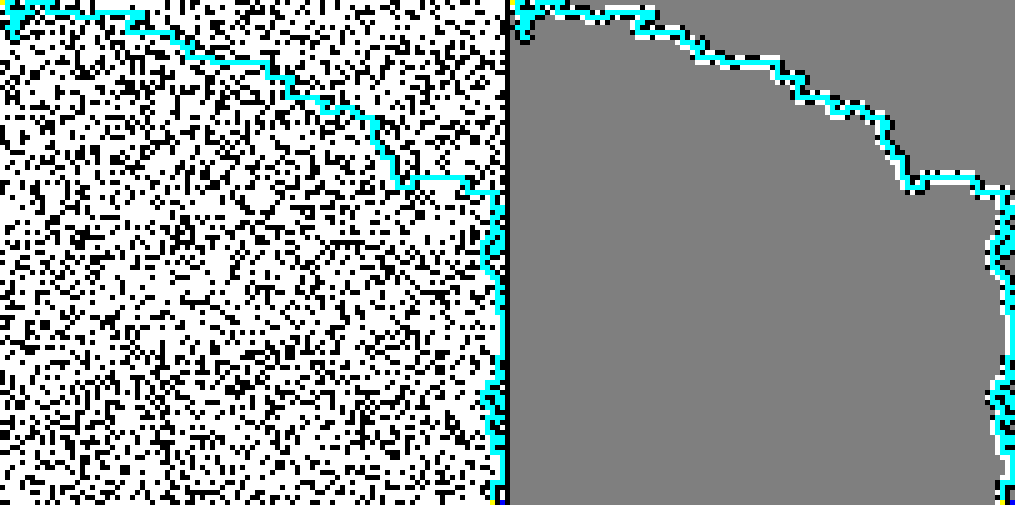
\includegraphics[width=0.85\textwidth]{q5-vis.png}
  \caption{Visualization of Adaptive A* on maze 3. The agent explored a corridor along the top-right of the grid before correctly determining the goal was unreachable. Grey indicates cells the agent never had reason to visit.}
\end{figure}

% -------------------------------------------------------
\section*{Part 6: Statistical Hypothesis Testing}

Performance differences between two algorithms observed on a finite set of test cases could be due to genuine algorithmic superiority or simply sampling noise from the particular mazes chosen. A statistical hypothesis test lets us distinguish between these possibilities.

\textbf{We describe a test for Part 2 (max\_g vs.\ min\_g):}

\textbf{Setup:} For each of the 50 mazes, we have a pair of measurements: the number of cells expanded by max\_g and the number expanded by min\_g on the same maze. Because the measurements are paired (same maze, different algorithm), we use a \textbf{paired t-test}.

\textbf{Hypotheses:}
\begin{itemize}
  \item $H_0$: The mean difference in expansions between min\_g and max\_g is zero (no systematic difference).
  \item $H_1$: The mean difference is not zero (one is systematically better).
\end{itemize}

\textbf{Procedure:}
\begin{enumerate}
  \item For each maze $i$, compute $d_i = \text{expansions}_{\text{min\_g},i} - \text{expansions}_{\text{max\_g},i}$.
  \item Compute the mean difference $\bar{d}$ and sample standard deviation $s_d$ over all 50 mazes.
  \item Compute the t-statistic: $t = \dfrac{\bar{d}}{s_d / \sqrt{50}}$.
  \item Compare $|t|$ to the critical value $t^* \approx 2.01$ at significance level $\alpha = 0.05$ with 49 degrees of freedom.
  \item If $|t| > t^*$, reject $H_0$ and conclude the difference is statistically significant.
\end{enumerate}

\textbf{Expected outcome:} The mean difference is $161{,}116 - 7{,}346 = 153{,}770$ expansions in favor of max\_g. Given this enormous magnitude and the consistency of the result (max\_g outperforms in 42 of 50 mazes), the t-statistic would be very large, and we would confidently reject $H_0$. The difference between max\_g and min\_g is not noise --- it is a systematic and statistically significant algorithmic advantage.

The same approach applies to Parts 3 and 5. For Part 5, the difference is smaller (265.8 expansions per solvable maze) but still consistent across 16 of 19 solvable mazes, which would likely also yield a significant result.

\end{document}